\begin{quote}
\textbf{Status:} draft $\cdot$ \textbf{Last updated:} 2026-11-22 $\cdot$
\textbf{Kind:} note (Slack post / tech-note draft)
\end{quote}

\subsection{Summary}\label{summary}

The Rubin Active Optics System (AOS) applies a hexapod look-up table
(LUT) in elevation and closes the loop on the corner wavefront sensors
(CWFS). This note measures what the LUT leaves uncorrected. It uses
pairs of science visits taken minutes apart that differ mainly in
elevation. The quantity measured is the open-loop optical state,
Deviation - Trim, in the 22-DOF, 12-mode (22/12) basis. It is compared
with the BLOCK-T720 A--B--A elevation bounce test, recovered in the same
basis.

\begin{itemize}
\tightlist
\item
  66,306 visit pairs on 107 nights, 20251209 to 20260713, all after the
  last LUT change.
\item
  Camera dx and camera rx give the largest and steadiest slopes: +10 to
  +12 $\mu$m per deg of elevation and +7 to +8 $\times$ 10$^{-5}$ deg per deg, in all
  three elevation bins.
\item
  Integrated from 70 deg down to 30 deg, the pairs give camera dx -421 $\pm$
  54 $\mu$m and camera rx -0.0031 $\pm$ 0.0002 deg. The bounce test gives -525 $\pm$
  107 $\mu$m and -0.0044 $\pm$ 0.0002 deg.
\item
  Over the 12 v-modes and 22 DOF, 31 of the 38 bounce slopes that are
  above 3$\sigma$ have the same sign as the pair slope. The pair slopes are
  smaller, with a median pair/bounce slope ratio of 0.14
  (dimensionless).
\item
  v-mode 1 (v1) and the defocus term DZ(1,4) disagree. The pairs give
  almost no net v1 change from 70 deg to 30 deg, while the bounce gives
  +0.019 (dimensionless).
\end{itemize}

\subsection{1. Method: paired science
visits}\label{method-paired-science-visits}

Two science visits on the same night form a pair when:

{ % do not increment counter
\begin{longtable}[]{@{}
  >{\raggedright\arraybackslash}p{(\linewidth - 2\tabcolsep) * \real{0.5000}}
  >{\raggedright\arraybackslash}p{(\linewidth - 2\tabcolsep) * \real{0.5000}}@{}}
\toprule\noalign{}
\begin{minipage}[b]{\linewidth}\raggedright
cut
\end{minipage} & \begin{minipage}[b]{\linewidth}\raggedright
value
\end{minipage} \\
\midrule\noalign{}
\endhead
\bottomrule\noalign{}
\endlastfoot
time between visit starts & $\le$ 5 min (the visits need not be
consecutive) \\
azimuth change, wrapped to $\pm$180 deg & \textbar $\Delta$Az\textbar{} \textless{}
5 deg \\
camera rotator angle change & \textbar $\Delta$Rot\textbar{} \textless{} 5
deg \\
band & unchanged \\
elevation change & \textbar $\Delta$El\textbar{} $\ge$ 2.5 deg \\
nights & day\_obs $\ge$ 20251209, the last hexapod LUT change \\
excluded nights & 20251210, 20251211, 20251212, 20251214, 20251216,
20251218, 20251219, 20260115, 20260116 (a different LUT setting) \\
wavefront & Danish 1.3 corner Zernikes on all four corner rafts at both
visits \\
\end{longtable}
}

Pointing, band and image type come from the Consolidated Database
(ConsDB). Holding azimuth, rotator angle and band fixed leaves elevation
as the main change across a pair. The short time separation limits
thermal drift.

The sample:

\begin{itemize}
\tightlist
\item
  72,669 science visits on 138 nights pass the night selection.
\item
  75,248 pairs pass the cuts, and 66,306 of them have a wavefront state
  at both visits. They span 107 nights and 42,321 distinct visits.
\item
  A visit is in 3.1 pairs on average, so pairs are not independent.
  There are 633 pairs per night (median).
\item
  Bands: i 17,815, z 16,091, y 12,839, r 11,410, g 5,545, u 2,606 pairs.
\item
  Most pairs come from survey blocks: BLOCK-407 has 50,294 pairs,
  BLOCK-421 6,588 and BLOCK-419 6,528.
\item
  The median time between visit starts is 1.9 min, and the median
  \textbar $\Delta$El\textbar{} is 4.7 deg.
\item
  \textbar $\Delta$El\textbar{} distribution: 37,123 pairs at 2.5--5 deg,
  25,259 at 5--10 deg, 3,826 at 10--20 deg and 98 above 20 deg.
\end{itemize}

The fits are done in three bins of the pair's midpoint elevation, (El$_1$ +
El$_2$)/2. The bins are 25--40 deg (6,356 pairs), 40--55 deg (25,424 pairs)
and 55--75 deg (33,963 pairs). 563 pairs fall outside 25--75 deg and are
in no bin.

\begin{figure}
\centering
\pandocbounded{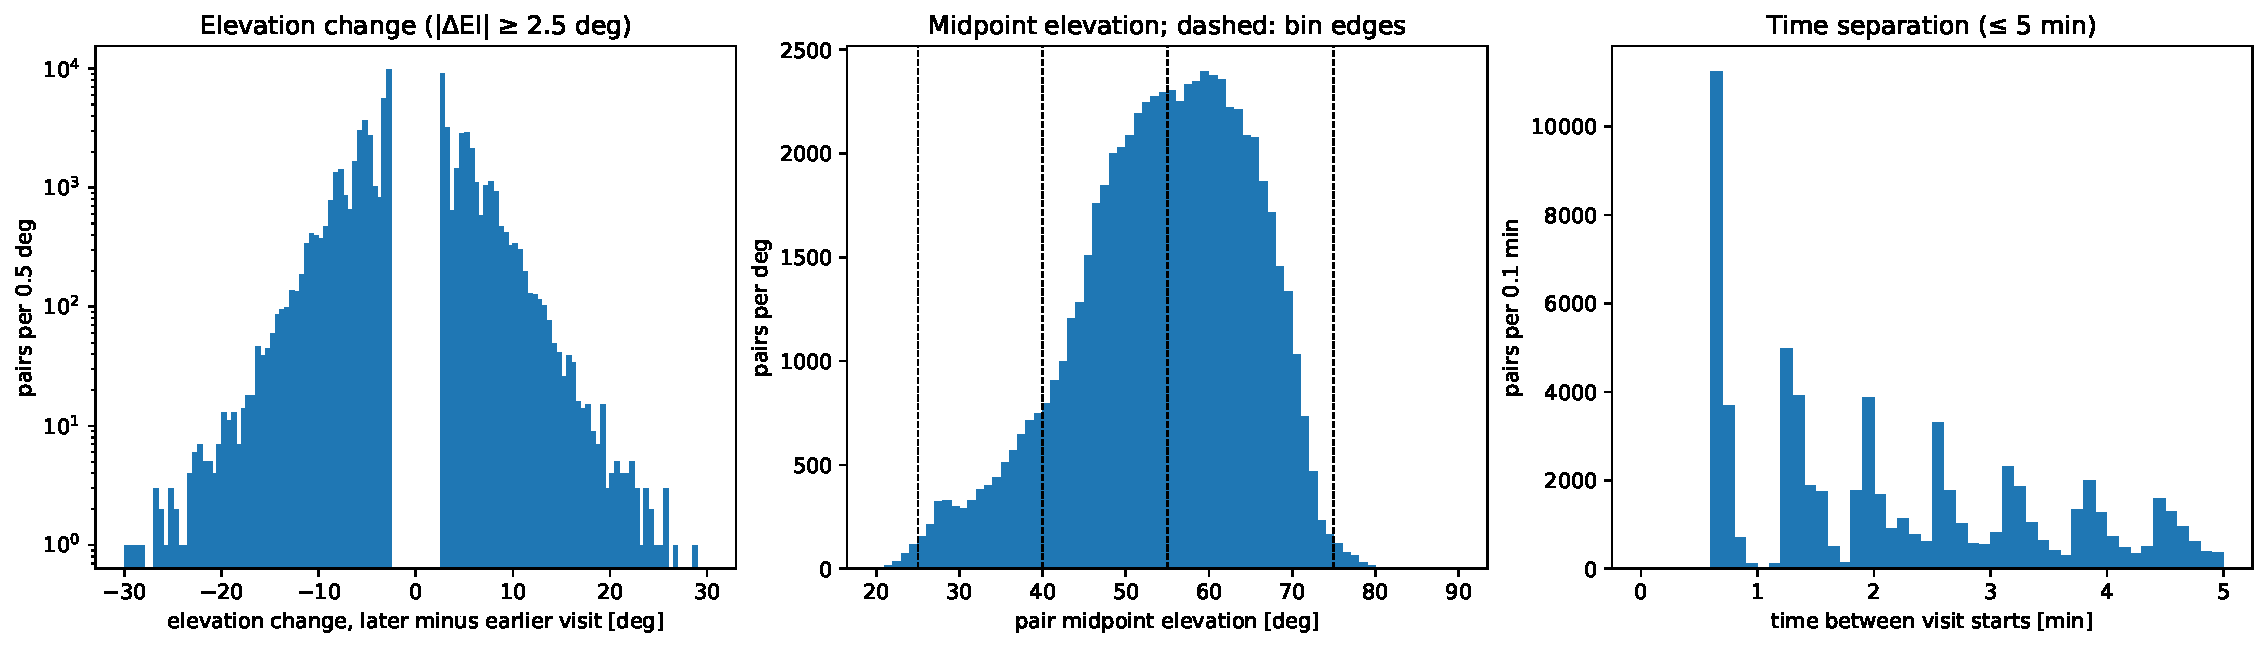
\includegraphics[keepaspectratio,alt={Pair sample. Left:
elevation change, later minus earlier visit; the gap is the 2.5 deg cut.
Centre: pair midpoint elevation, with the bin edges dashed. Right: time
between the two visit starts.}]{figures/fig01_sample}}
\caption{Pair sample. Left: elevation change, later minus earlier visit;
the gap is the 2.5 deg cut. Centre: pair midpoint elevation, with the
bin edges dashed. Right: time between the two visit starts.}
\end{figure}

\subsection{2. Optical state: Deviation -
Trim}\label{optical-state-deviation-trim}

For each visit, two sets of degrees of freedom (DOF) are combined:

\begin{itemize}
\tightlist
\item
  \textbf{Trim}: the DOF correction commanded by the AOS. It is read
  from the Engineering Facilities Database (EFD) topic
  \texttt{MTAOS.logevent\_degreeOfFreedom} as of the visit start,
  through the \texttt{value\_added} DuckDB database of per-exposure
  telemetry. Its units are $\mu$m, and deg for hexapod tilts.
\item
  \textbf{Deviation}: the DOF recovered from the wavefront measured on
  the corner sensors in the same visit.
\end{itemize}

The open-loop state is \textbf{Deviation - Trim}: the wavefront the
telescope would have had with the loop open. It does not include the
hexapod LUT, which is applied in both visits. Its change across a pair
is therefore the part of the elevation dependence that the LUT leaves
uncorrected. The A--B--A bounce test measures the same quantity with the
same sign.

The deviation comes from this processing:

{ % do not increment counter
\begin{longtable}[]{@{}
  >{\raggedright\arraybackslash}p{(\linewidth - 2\tabcolsep) * \real{0.5000}}
  >{\raggedright\arraybackslash}p{(\linewidth - 2\tabcolsep) * \real{0.5000}}@{}}
\toprule\noalign{}
\begin{minipage}[b]{\linewidth}\raggedright
step
\end{minipage} & \begin{minipage}[b]{\linewidth}\raggedright
setting
\end{minipage} \\
\midrule\noalign{}
\endhead
\bottomrule\noalign{}
\endlastfoot
wavefront estimation & Danish 1.3 (\texttt{danish\_1\_3\_0}) \\
corner task & blitz (\texttt{donutBlitzCornerResults}), unpaired: each
corner half-chip fitted on its own \\
binning, pupil model & 2 $\times$ 2 binned images, v3.14 pupil model \\
processing run & RSO-1071 science reprocessing, collection
\texttt{LSSTCam/runs/aos/cwfs/danish\_1\_3\_0/wep\_blitz\_rso1071/dv\_blitz\_rso1071/bin\_x2/unpaired/donutBlitz} \\
product & \texttt{cwfs\_science} variant \texttt{d13-blitz\_rso1071},
build 20261026 \\
donut selection & the product's quality cut: a pipeline candidate with a
successful (\texttt{ok}) fit and finite SNR, blur and Zernikes \\
per half-chip & median Zernike over the selected donuts, minus the
intrinsic (batoid model) wavefront, in the Optical Coordinate System
(OCS) \\
per raft & mean of the extra-focal (SW0) and intra-focal (SW1)
half-chips; a raft needs both \\
state recovery & \texttt{aos\_state.recover\_optical\_state}, ts\_ofc
v13 sensitivity matrix, DOF set \texttt{standard\_22}, 12 v-modes kept
(22/12) \\
\end{longtable}
}

The 22 DOF are: - the 10 hexapod DOF: M2 and camera dz, dx, dy ($\mu$m) and
rx, ry (deg); - M1M3 (primary/tertiary mirror) bending modes B1--B7
($\mu$m); - M2 (secondary mirror) bending modes B1--B5 ($\mu$m).

The v-modes are the 12 singular vectors of the normalized sensitivity
matrix in that DOF set (dimensionless).

\textbf{Fit.} For each quantity X (a v-mode or a DOF), the change $\Delta$X =
X(later visit) - X(earlier visit) is fitted against $\Delta$El with a Huber
robust line, $\Delta$X = a + b $\Delta$El, using statsmodels \texttt{RLM} with
\texttt{HuberT}. The slope b, in units of X per deg, is the elevation
derivative at the bin's midpoint elevation.

\textbf{Errors.} Pairs share visits and nights, so the formal Huber
errors are too small. The errors quoted are night-clustered sandwich
errors, which treat each night as one independent unit. A 200-resample
night bootstrap of v1 and DZ(1,4) agrees with them to within 10\%. The
clustered errors are 2.3 to 7.3 times the formal ones (dimensionless
ratio, over all quantities and bins).

\subsection{3. Examples: camera dx and camera
rx}\label{examples-camera-dx-and-camera-rx}

Camera dx and camera rx show the clearest elevation dependence. Their
slopes are about the same in all three bins, so the LUT residual in
these two DOF is close to linear in elevation.

{ % do not increment counter
\begin{longtable}[]{@{}
  >{\raggedright\arraybackslash}p{(\linewidth - 4\tabcolsep) * \real{0.3333}}
  >{\raggedright\arraybackslash}p{(\linewidth - 4\tabcolsep) * \real{0.3333}}
  >{\raggedright\arraybackslash}p{(\linewidth - 4\tabcolsep) * \real{0.3333}}@{}}
\toprule\noalign{}
\begin{minipage}[b]{\linewidth}\raggedright
midpoint elevation {[}deg{]}
\end{minipage} & \begin{minipage}[b]{\linewidth}\raggedright
camera dx slope {[}$\mu$m/deg{]}
\end{minipage} & \begin{minipage}[b]{\linewidth}\raggedright
camera rx slope {[}10$^{-5}$ deg/deg{]}
\end{minipage} \\
\midrule\noalign{}
\endhead
\bottomrule\noalign{}
\endlastfoot
25--40 & +12.0 $\pm$ 3.2 & +7.7 $\pm$ 1.4 \\
40--55 & +10.2 $\pm$ 2.0 & +7.0 $\pm$ 0.7 \\
55--75 & +9.9 $\pm$ 2.1 & +8.3 $\pm$ 0.5 \\
\end{longtable}
}

Single-pair scatter is large: the camera dx change has a spread of about
$\pm$1000 $\mu$m at fixed $\Delta$El. The slope is still well measured, because there
are tens of thousands of pairs. The correlations are weak: for camera
dx, Pearson r is +0.05 to +0.11 and Spearman $\rho$ is +0.10 to +0.13 (n as
in each panel).

\begin{figure}
\centering
\pandocbounded{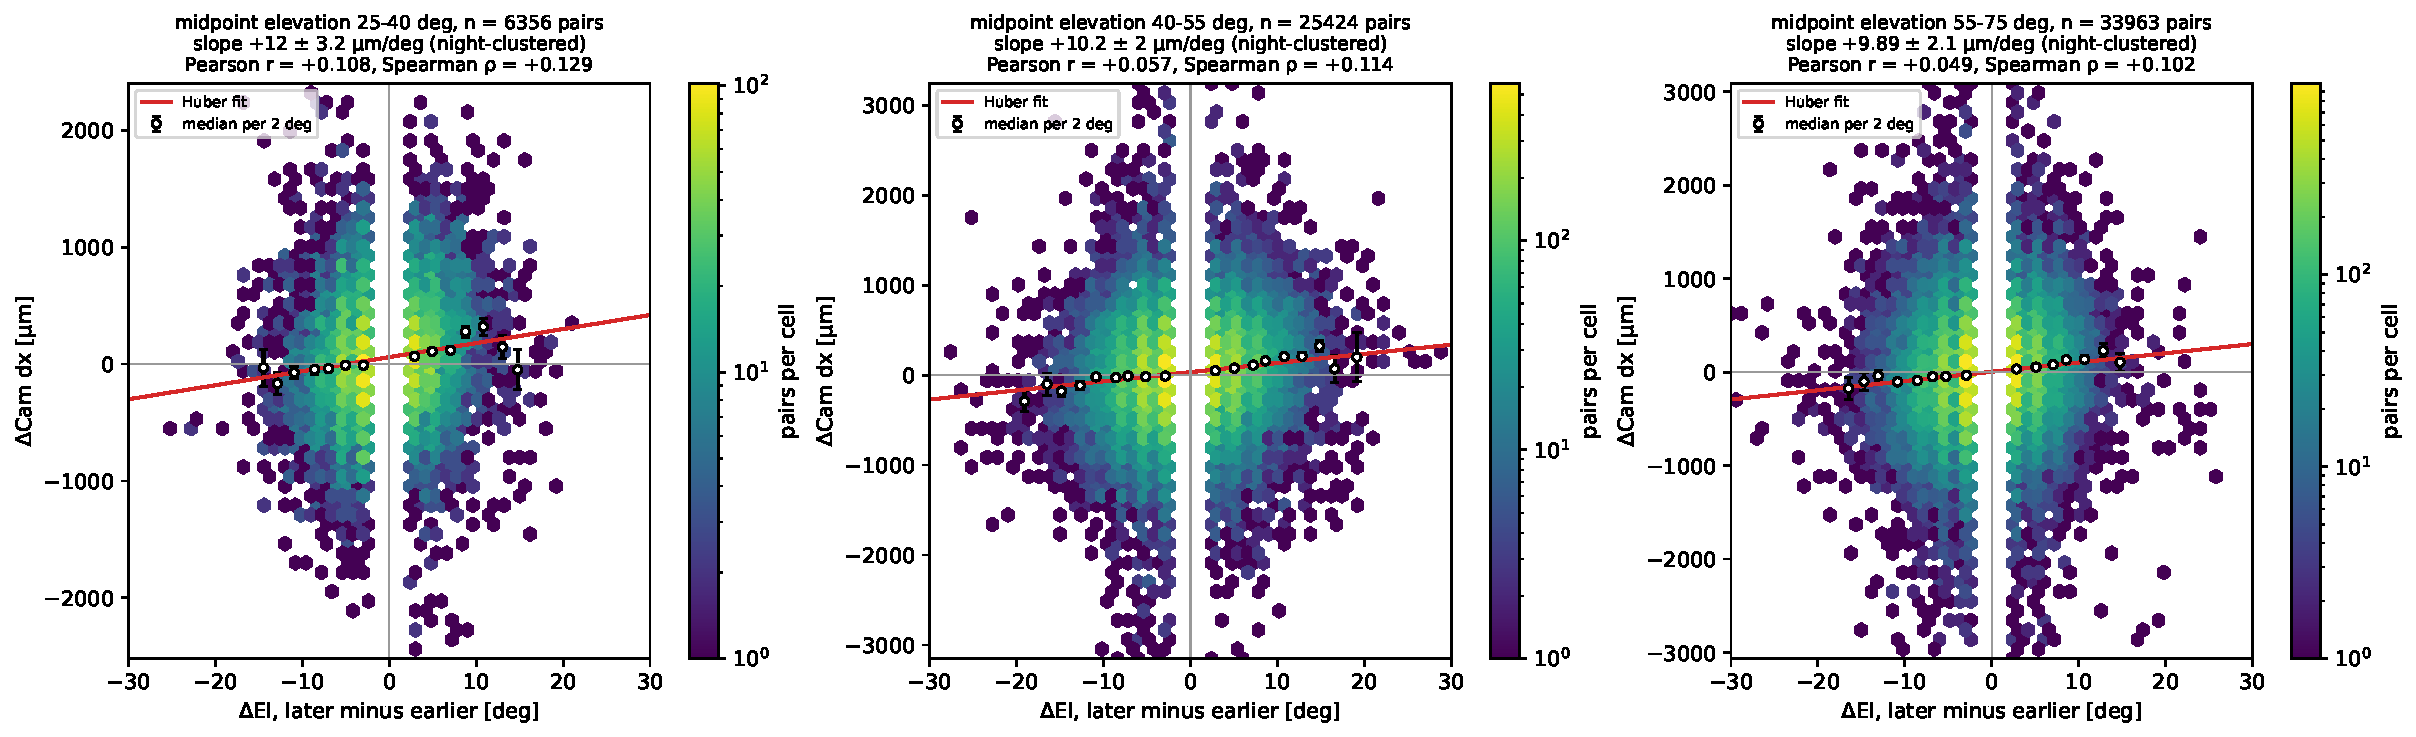
\includegraphics[keepaspectratio,alt={Camera dx change
against elevation change, Deviation - Trim, in the three
midpoint-elevation bins. Colour: pairs per hexbin cell (log scale).
White points: median per 2 deg of $\Delta$El. Red: Huber
fit.}]{figures/fig02_cam_dx_bins}}
\caption{Camera dx change against elevation change, Deviation - Trim, in
the three midpoint-elevation bins. Colour: pairs per hexbin cell (log
scale). White points: median per 2 deg of $\Delta$El. Red: Huber fit.}
\end{figure}

\begin{figure}
\centering
\pandocbounded{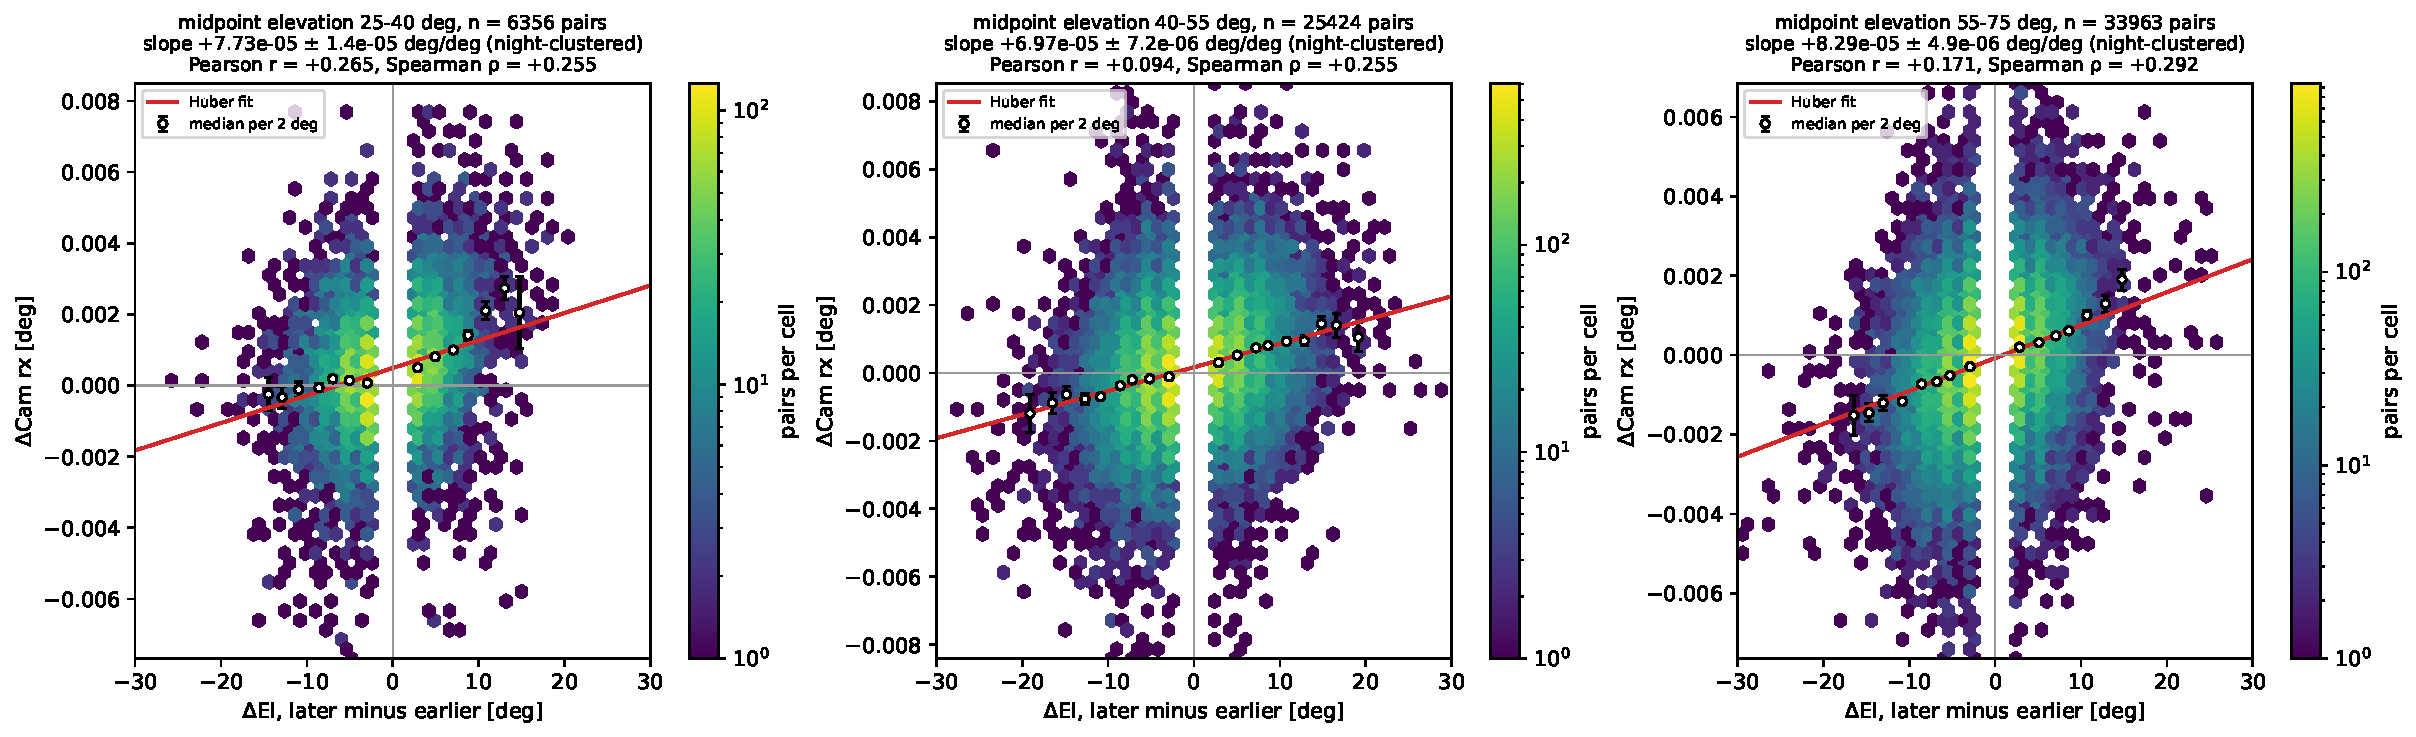
\includegraphics[keepaspectratio,alt={Camera rx change
against elevation change, as in the previous
figure.}]{figures/fig03_cam_rx_bins}}
\caption{Camera rx change against elevation change, as in the previous
figure.}
\end{figure}

\subsection{4. Comparison with the A--B--A bounce
test}\label{comparison-with-the-aba-bounce-test}

The bounce test is BLOCK-T720, an elevation sweep with the loop frozen.
Its reference visits (A) are at 70 deg, and between them are test visits
(B) at 30, 40, 50, 60 and 75 deg.

\begin{itemize}
\tightlist
\item
  Each leg is B - A, with A interpolated in time to the B visit. It is
  measured from Full Array Mode (FAM) double Zernikes (DZ) with the
  batoid intrinsic subtracted.
\item
  The leg is recovered in the same 22/12 basis, from the
  \texttt{bounce\_aba} product, variant \texttt{d13-batoid-22\_12},
  build 20261121.
\item
  The errors come from a Monte Carlo noise model fitted to the same
  visits.
\item
  The legs were taken on six nights: 40 deg on 20260418, 20260419 and
  20260513, 60 deg on 20260709, 50 deg on 20260711, and 30 and 75 deg on
  20260713.
\end{itemize}

In each panel below, the black points are the bounce B - A values, and
the open circle is the 70 deg reference, zero by definition. Each
coloured segment is a pair slope. It spans its midpoint-elevation bin
and is anchored on the bounce curve, interpolated at the bin centre, so
only its slope is compared. The bands are $\pm$1$\sigma$.

\begin{figure}
\centering
\pandocbounded{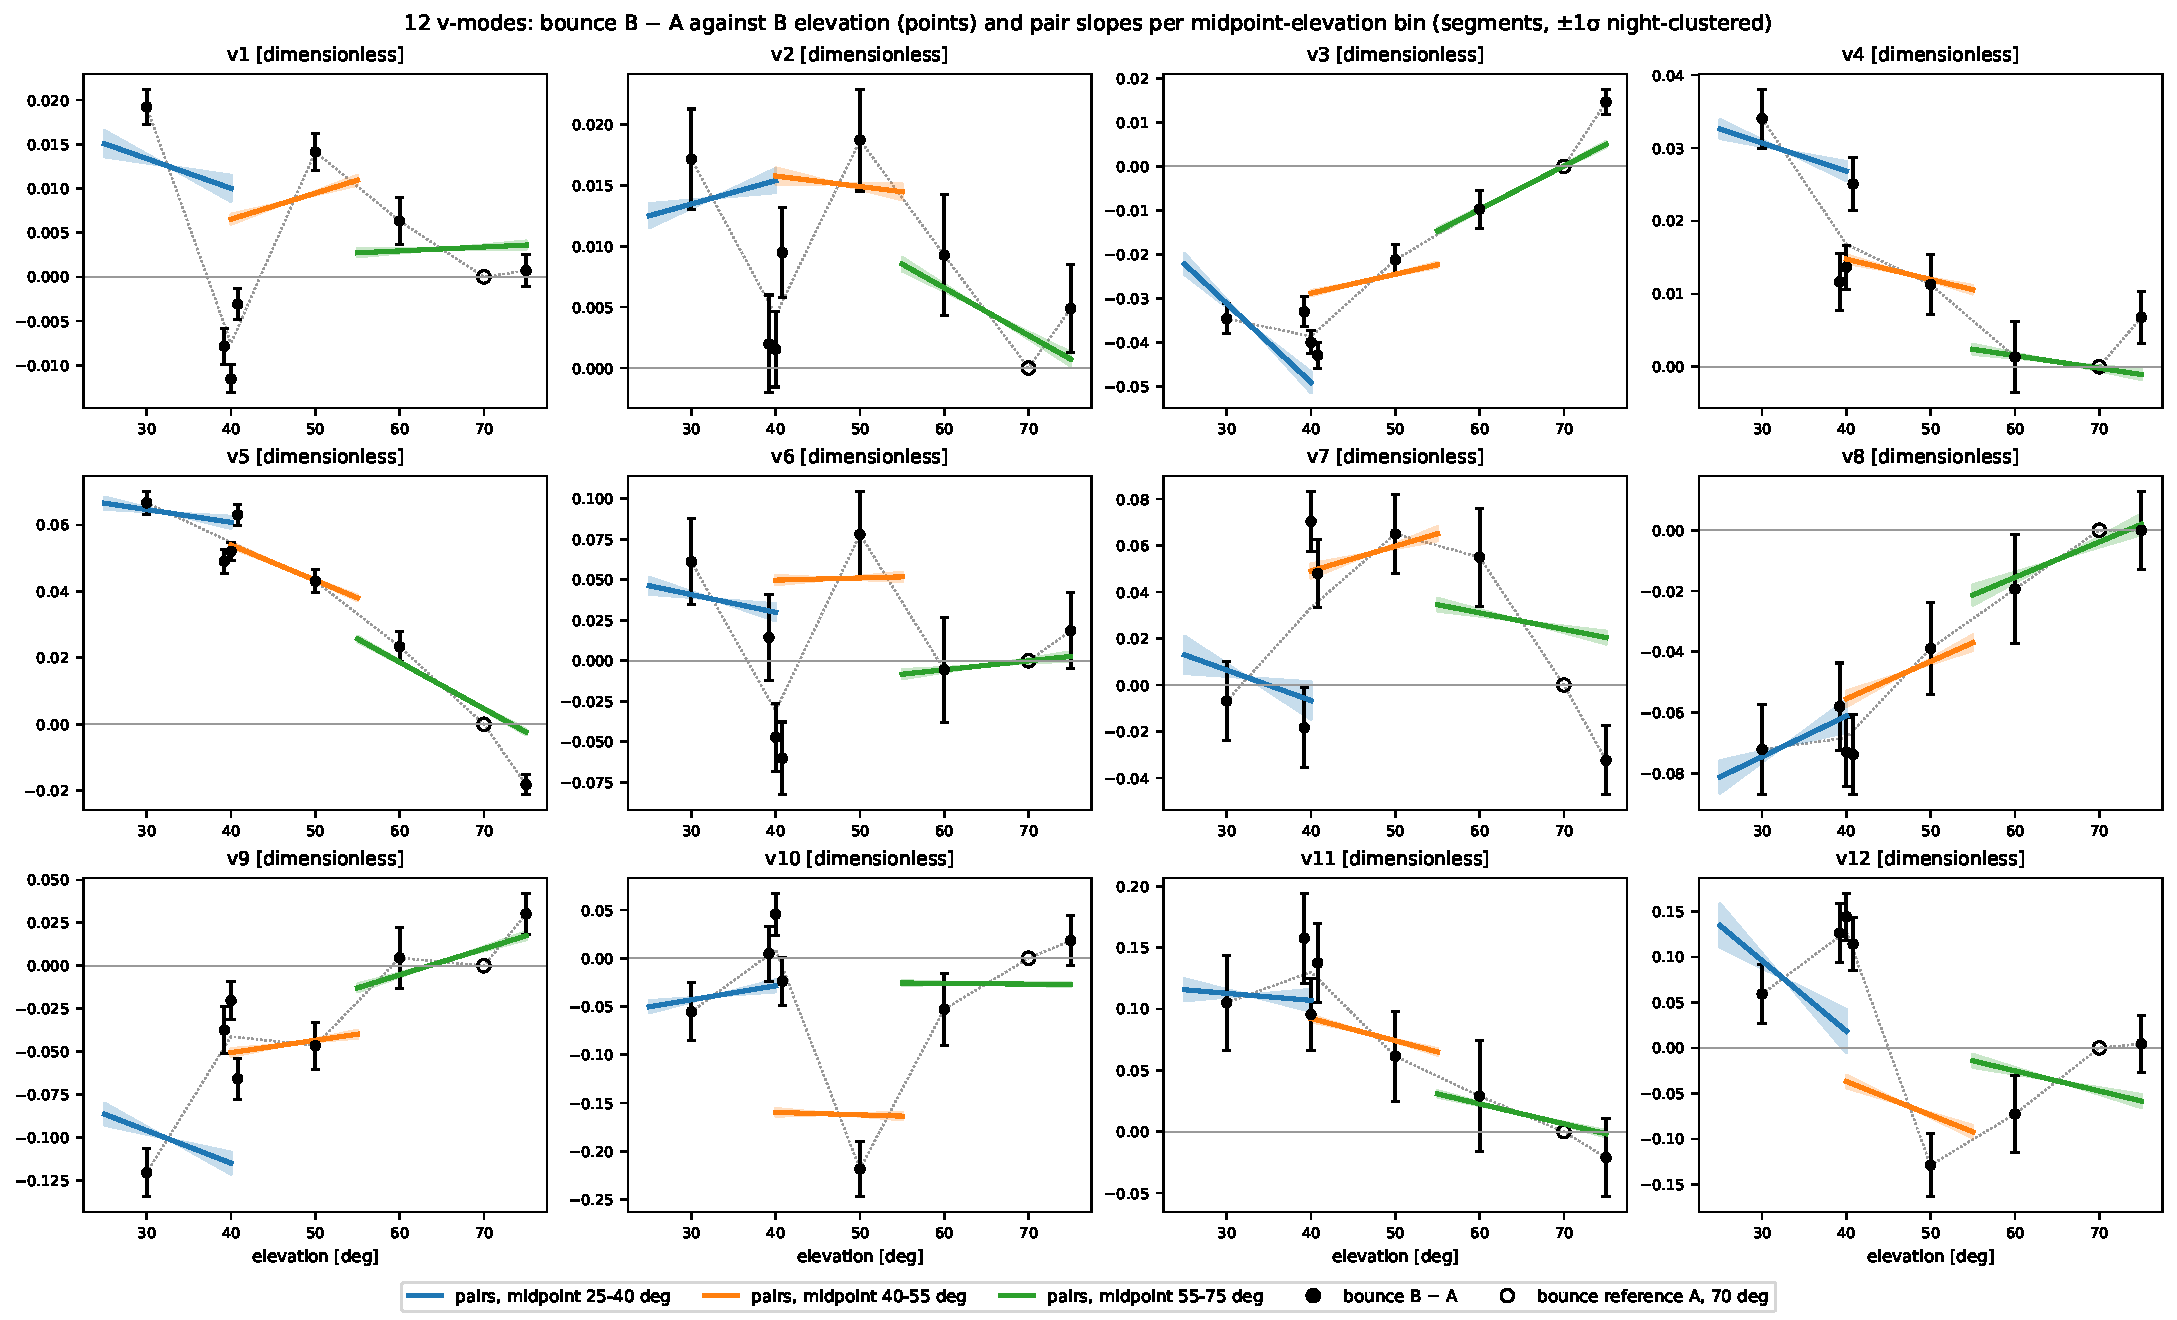
\includegraphics[keepaspectratio,alt={The 12 v-modes
(dimensionless): bounce B - A against B elevation, and pair slopes per
midpoint-elevation bin.}]{figures/fig04_vmodes_bounce}}
\caption{The 12 v-modes (dimensionless): bounce B - A against B
elevation, and pair slopes per midpoint-elevation bin.}
\end{figure}

\begin{figure}
\centering
\pandocbounded{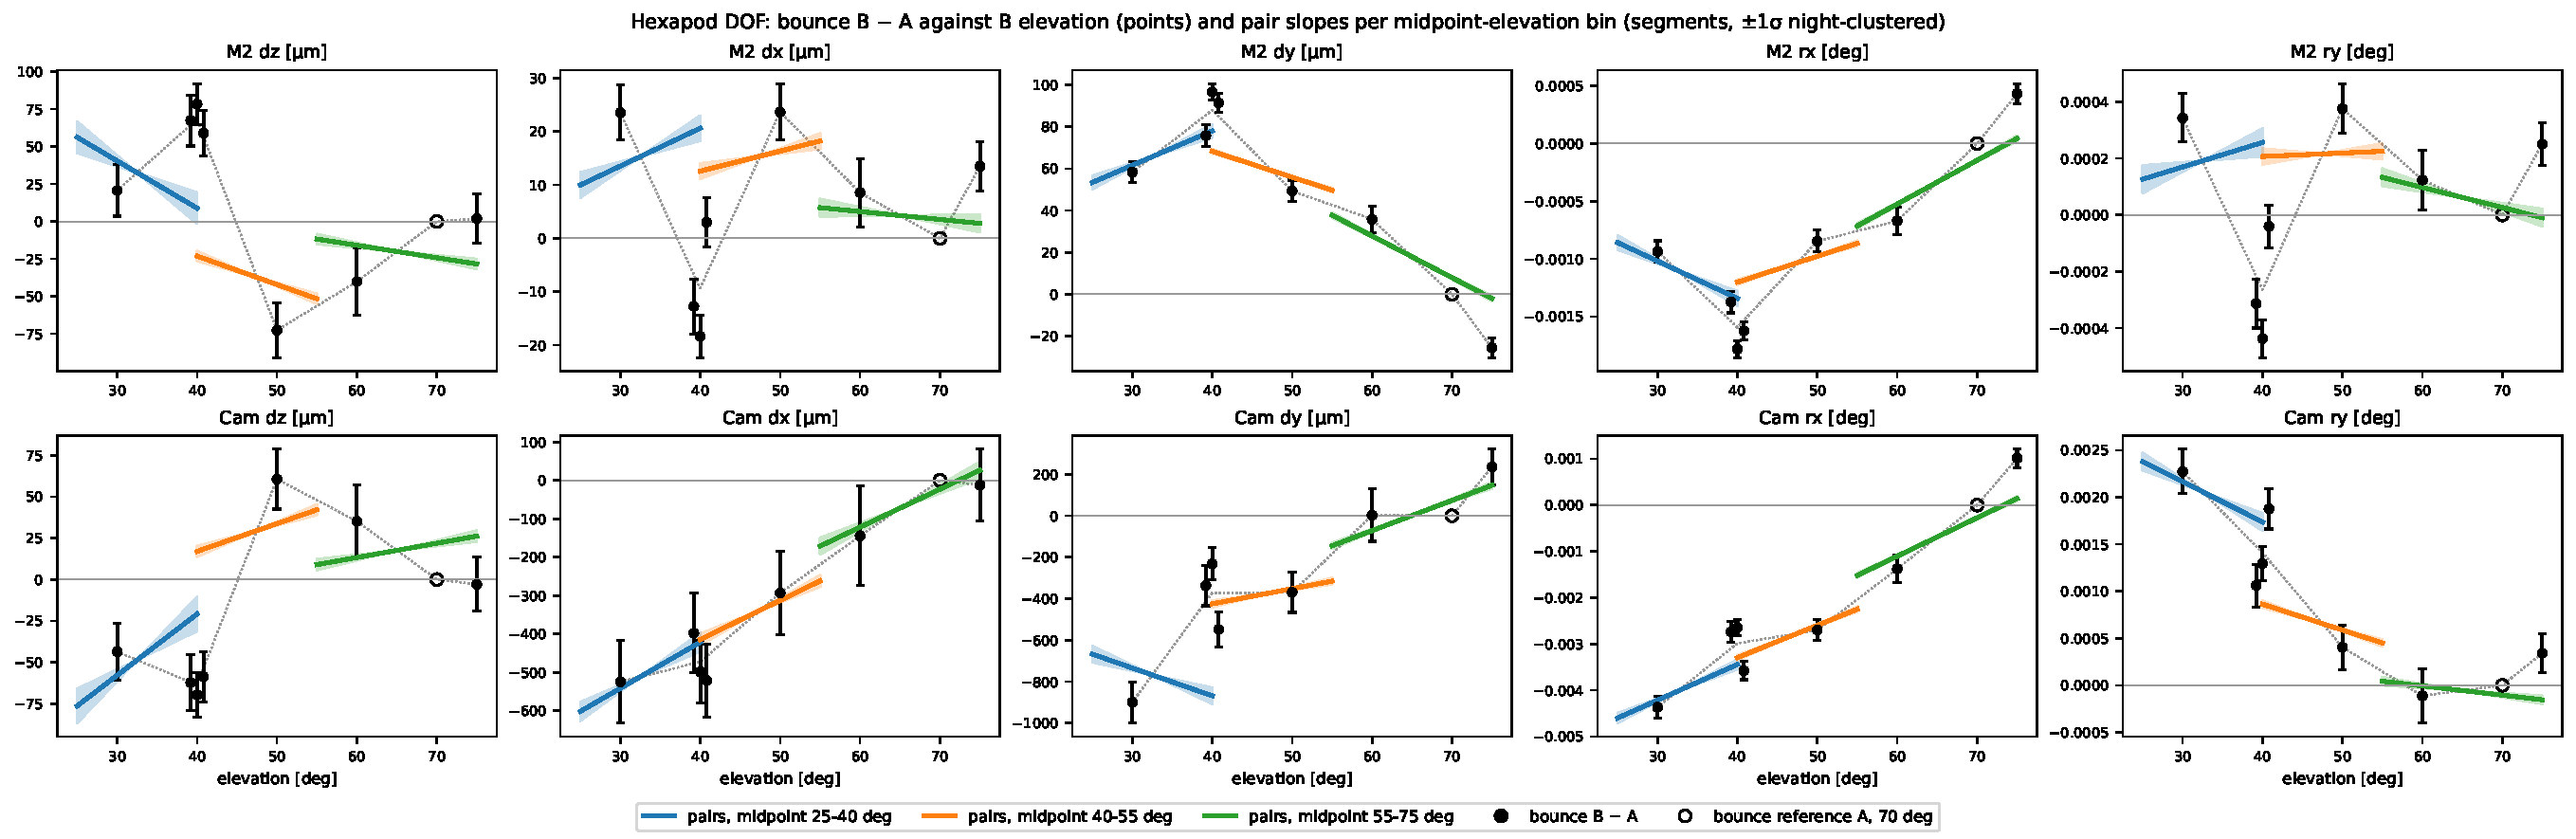
\includegraphics[keepaspectratio,alt={The 10 hexapod DOF
($\mu$m; rx and ry in deg).}]{figures/fig05_hexapods_bounce}}
\caption{The 10 hexapod DOF ($\mu$m; rx and ry in deg).}
\end{figure}

\begin{figure}
\centering
\pandocbounded{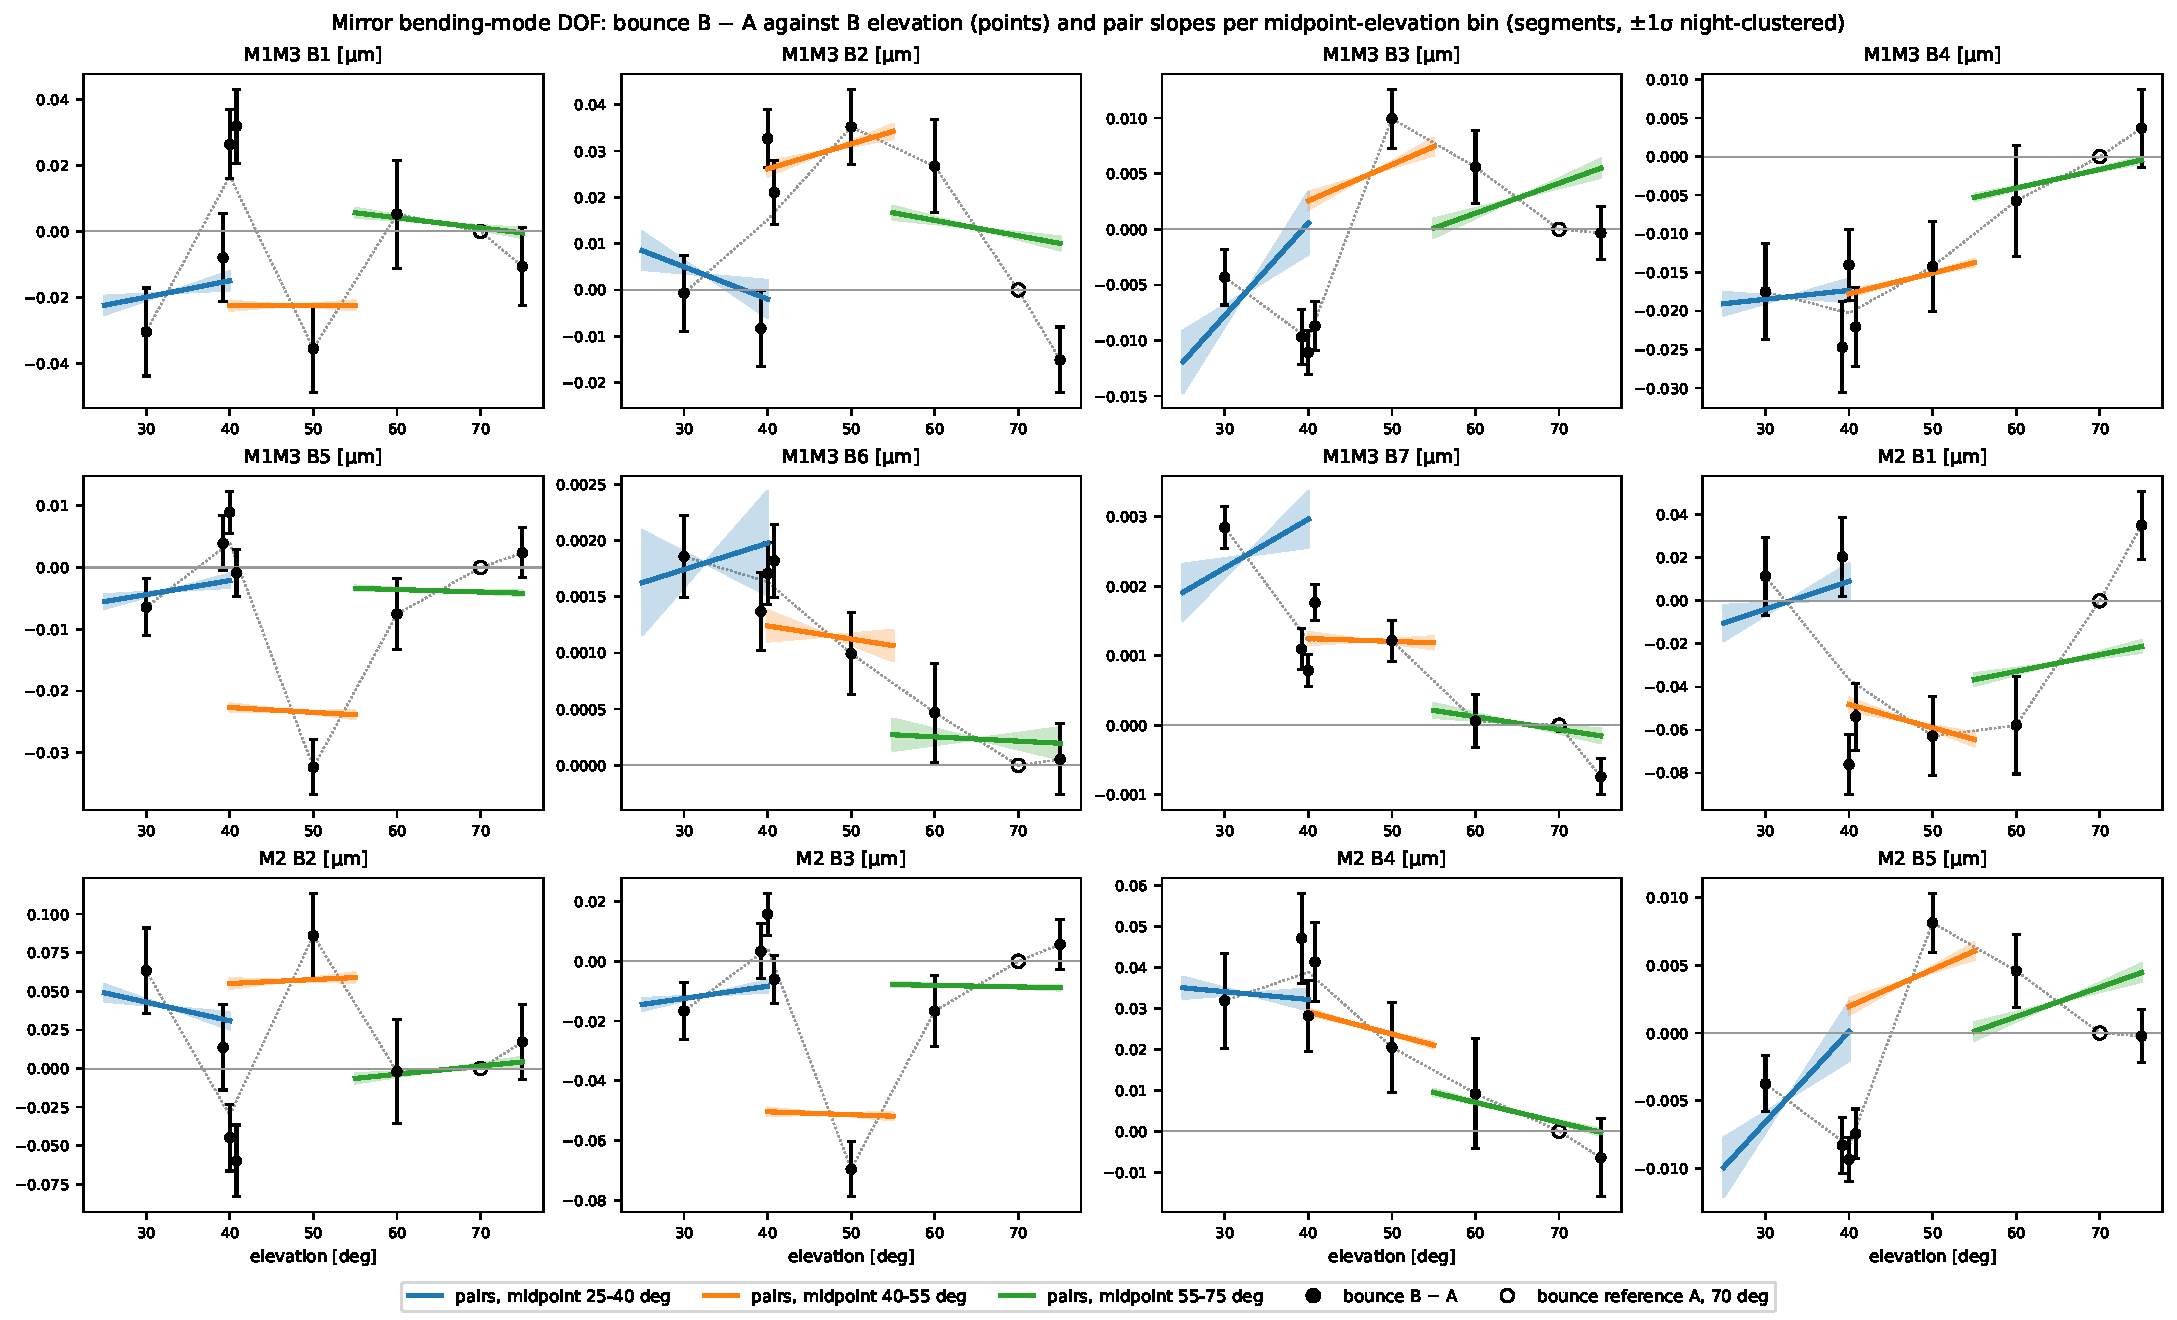
\includegraphics[keepaspectratio,alt={The 12 mirror
bending-mode DOF in the 22/12 set: M1M3 B1--B7 and M2 B1--B5
($\mu$m).}]{figures/fig06_bending_bounce}}
\caption{The 12 mirror bending-mode DOF in the 22/12 set: M1M3 B1--B7
and M2 B1--B5 ($\mu$m).}
\end{figure}

Bounce slopes between legs were computed at 30--40, 40--50 and 60--70
deg, with the three 40 deg nights averaged. They were compared with the
pair slopes in the 25--40, 40--55 and 55--75 deg bins. Of the 38 bounce
slopes above 3$\sigma$, 31 have the pair slope's sign. The median pair/bounce
slope ratio is 0.14 (dimensionless).

Pair slopes summed from 0 at 70 deg down to 30 deg, against the 30 deg
bounce leg:

{ % do not increment counter
\begin{longtable}[]{@{}llll@{}}
\toprule\noalign{}
DOF or mode & unit & pairs & bounce, 20260713 \\
\midrule\noalign{}
\endhead
\bottomrule\noalign{}
\endlastfoot
camera dx & $\mu$m & -421 $\pm$ 54 & -525 $\pm$ 107 \\
camera rx & deg & -0.0031 $\pm$ 0.0002 & -0.0044 $\pm$ 0.0002 \\
camera ry & deg & +0.0010 $\pm$ 0.0002 & +0.0023 $\pm$ 0.0002 \\
M2 dy & $\mu$m & +32 $\pm$ 5 & +58 $\pm$ 5 \\
camera dy & $\mu$m & -194 $\pm$ 64 & -900 $\pm$ 99 \\
M2 dz & $\mu$m & +73 $\pm$ 16 & +21 $\pm$ 17 \\
camera dz & $\mu$m & -75 $\pm$ 16 & -44 $\pm$ 17 \\
v1 & dimensionless & -0.002 $\pm$ 0.002 & +0.019 $\pm$ 0.002 \\
\end{longtable}
}

Camera dx agrees within errors. Camera rx, camera ry and M2 dy have the
right sign at 50\% to 70\% of the bounce value. Camera dy and v1
disagree. In the 22/12 basis, M2 dz and camera dz each change by many
tens of $\mu$m in opposite directions, and their sum sets v1; the pairs and
the bounce split that sum differently.

\subsection{5. Caveats}\label{caveats}

\begin{itemize}
\tightlist
\item
  \textbf{The bounce legs come from different nights.} Only 20260713 has
  two legs, 30 and 75 deg. A bounce slope between legs mixes elevation
  with night-to-night changes. The zigzag at 40 deg in v1 and several
  DOF suggests this effect.
\item
  \textbf{The wavefront sensors differ.} The pairs use the four corner
  sensors in science visits, and the bounce uses FAM on the science
  sensors. Both are fitted in the same 22/12 basis, but the corner
  sensors constrain the field dependence less well.
\item
  \textbf{At 55--75 deg the small-$\Delta$El pairs depart from the line.} The
  DZ(1,4) slope there is -0.0020 $\pm$ 0.0007 $\mu$m of wavefront per deg at
  \textbar $\Delta$El\textbar{} 2.5--5 deg, against +0.0004 $\pm$ 0.0007 at 5--10
  deg. This bin holds half the pairs, so its slopes for v1 and the dz
  DOF should be read with that in mind.
\item
  \textbf{DZ in the pairs is a projection.} It is S(k,j) times the 22
  recovered DOF, where S is the sensitivity matrix, so it holds only the
  12-mode part of the measured wavefront.
\end{itemize}

\subsection{Provenance}\label{provenance}

Products, builds, code versions and how to regenerate the figures are in
\url{provenance.md}. The analysis is the \texttt{aos/elevation\_pairs}
study.
